% =============================================================================
%  BEAMER TEMPLATE
%  ---------------------------------------------------------------------------
%  This is the only file you normally need to touch to start a new deck.
%  Fill in the metadata block, then write your content in Sections/.
% =============================================================================
\documentclass[10pt, aspectratio=169]{beamer}

\usepackage{Preamble/preamble}
% =============================================================================
%  BRANDING  --  edit the four lines below and the whole deck follows.
% =============================================================================
\definecolor{BrandPrimary}{RGB}{36, 164, 220}   % main colour (bars, section dividers)
\definecolor{BrandAccent}{RGB}{201, 42, 135}    % accent (alerts, highlights)
\definecolor{BrandDark}{RGB}{0, 33, 71}         % dark text / contrast
\newcommand{\brandlogo}{Assets/logo.png}        % empty {} to hide the logo
% =============================================================================

% --- Beamer colours ---------------------------------------------------------
\setbeamercolor{palette primary}{bg=BrandPrimary, fg=white}
\setbeamercolor{structure}{fg=BrandPrimary}
\setbeamercolor{titlelike}{fg=BrandPrimary}
\setbeamercolor{frametitle}{bg=BrandPrimary, fg=white}
\setbeamercolor{alerted text}{fg=BrandAccent}
\setbeamercolor{block title}{bg=BrandPrimary!15, fg=BrandDark}
\setbeamercolor{block body}{bg=BrandPrimary!5}

% --- Links ------------------------------------------------------------------
% Deferred to \begin{document} so hyperref is guaranteed to be loaded already.
\AtBeginDocument{%
  \hypersetup{
    colorlinks=true,
    linkcolor=BrandPrimary,
    urlcolor=BrandPrimary,
    citecolor=BrandPrimary
  }%
}


% -----------------------------------------------------------------------------
%  1. DECK METADATA  --  change these five lines
% -----------------------------------------------------------------------------
\title{Presentation Title}
\subtitle{Optional subtitle}                   % leave {} to hide
\author{Your Name}
\institute{University -- Faculty}
\renewcommand{\courseline}{Course code -- Group X}  % leave {} to hide
\date{\today}                                 % or e.g. {May 1, 2026}

\begin{document}

% -----------------------------------------------------------------------------
%  2. TITLE SLIDE  (rendered from the metadata above)
% -----------------------------------------------------------------------------
% =============================================================================
%  TITLE SLIDE
%  Everything here comes from main.tex; no text is hard-coded.
%  Sizes are tuned so the whole stack (title card + metadata + logo) fits on
%  a 16:9 slide without pushing the logo off the bottom edge.
% =============================================================================
\begin{frame}[plain]
    \centering

    % --- Title card ---------------------------------------------------------
    \begin{tcolorbox}[
        enhanced,
        colback=BrandPrimary,
        colframe=BrandPrimary,
        arc=10pt,
        boxrule=0pt,
        width=0.95\paperwidth,
        center,
        shadow={2pt}{-2pt}{0pt}{black!30},
        halign=flush right,
        valign=center,
        height=2.6cm,
        right=0.8cm,
        after skip=0pt
    ]
        {\fontsize{24}{28}\selectfont\bfseries\color{white}%
         \inserttitle
         \ifx\insertsubtitle\empty\else
             \\[0.1cm]{\fontsize{14}{17}\selectfont\normalfont\insertsubtitle}%
         \fi
         \par}
    \end{tcolorbox}

    \vspace{0.45cm}

    % --- Course / group line (optional) ------------------------------------
    \ifx\courseline\empty\else
        {\Large\bfseries\color{BrandPrimary} \courseline}\\[0.18cm]
    \fi

    % --- Author and institute ----------------------------------------------
    {\large \insertauthor} \\[0.1cm]
    {\normalsize \insertinstitute}

    \vspace{0.25cm}

    % --- Date ---------------------------------------------------------------
    {\small \insertdate}

    \vfill

    % --- Logo (only if the file exists) ------------------------------------
    \IfFileExists{\brandlogo}{%
        \includegraphics[height=1cm, keepaspectratio]{\brandlogo}%
    }{}
    \vspace{0.25cm}
\end{frame}


% -----------------------------------------------------------------------------
%  3. AGENDA
% -----------------------------------------------------------------------------
% =============================================================================
%  AGENDA
%  Filled automatically from \section[...]{...} in every section file.
% =============================================================================
\begin{frame}{Agenda}
    \tableofcontents
\end{frame}


% -----------------------------------------------------------------------------
%  4. CONTENT
%     Each section file declares its own \section at the top, so the section
%     divider slide and the agenda update automatically.
% -----------------------------------------------------------------------------
% =============================================================================
%  SECTION 01 -- DEMO
%  Replace the frames below with your own content, or delete this file and
%  point main.tex at a new one. The section divider slide is generated
%  automatically from \section[short]{long}.
% =============================================================================
\section[Demo Section]{Demo Section}

\begin{frame}{A slide with nested bullets}
    \begin{itemize}
        \item A first-level point
        \begin{itemize}
            \item A supporting detail
            \item Another detail with \alert{highlighted text}
        \end{itemize}

        \item A second first-level point
        \begin{itemize}
            \item \textbf{Bold lead-in:} the explanation of the idea.
            \item Inline code looks like \texttt{this}.
        \end{itemize}
    \end{itemize}
\end{frame}

\begin{frame}{Text and image side by side}
    \begin{columns}[T, onlytextwidth]
        \begin{column}{0.52\textwidth}
            \begin{itemize}
                \item Put prose on one side
                \item Put a figure, diagram or table on the other
                \item Change the two widths to rebalance the slide
            \end{itemize}
        \end{column}

        \begin{column}{0.44\textwidth}
            \centering
            % Replace the placeholder with a real image:
            %   \includegraphics[width=\linewidth]{Assets/your-image.png}
            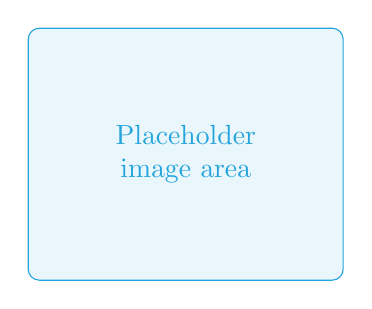
\begin{tikzpicture}
                \node[draw=BrandPrimary, fill=BrandPrimary!10, rounded corners,
                      minimum width=4cm, minimum height=3.2cm, align=center,
                      text=BrandPrimary]
                    {Placeholder\\image area};
            \end{tikzpicture}
        \end{column}
    \end{columns}
\end{frame}

\begin{frame}{Callout box}
    \begin{itemize}
        \item A normal bullet for context
        \item Choose boxes over bold paragraphs when one message matters most
    \end{itemize}

    \vspace{0.3cm}

    \begin{tcolorbox}[colback=BrandPrimary!8, colframe=BrandPrimary,
                      boxrule=0.6pt, arc=3pt, left=6pt, right=6pt]
        \textbf{Key idea.} Definitions, warnings and single takeaways belong in
        a box like this one so the audience can find them at a glance.
    \end{tcolorbox}
\end{frame}


% -----------------------------------------------------------------------------
%  5. CLOSING  --  delete the next line to end without a thank-you slide
% -----------------------------------------------------------------------------
% =============================================================================
%  CLOSING SLIDE
%  Delete the matching \input in main.tex to drop this slide.
% =============================================================================
\begin{frame}[plain]
    \centering
    \vfill

    {\Huge\bfseries\color{BrandPrimary} Thank you}\\[0.4cm]
    {\Large Questions \& Discussion}

    \vfill

    \IfFileExists{\brandlogo}{%
        \includegraphics[height=1.2cm, keepaspectratio]{\brandlogo}%
    }{}
    \vspace{0.5cm}
\end{frame}


\end{document}
